\documentclass[]{article}

\usepackage[T1]{fontenc}
\usepackage{textcomp}

\usepackage{parskip}
\usepackage{listings}
\lstset{upquote=true}

\usepackage[sorting=ynt]{biblatex}
\addbibresource{general.bib}

\usepackage[x11names]{xcolor}
\usepackage{hyperref}
\hypersetup{breaklinks}
\hypersetup{colorlinks}
% Tone down hyperref's garish default colors
\hypersetup{citecolor=SpringGreen4}
\hypersetup{urlcolor=blue}

\usepackage{csquotes}
\MakeOuterQuote{"}

\usepackage{tikz}

\def\handoutdate{Tue Oct 13, 2020}
\def\deadline{Tue Nov 03, 2020 at 12:15 (start of colloquium period)}

\title{%
INF-3200: Distributed Systems Fundamentals \\
Fall 2020 \\
Mandatory Assignment 2: Membership \\
}
\author{Mike Murphy \and Aakash Sharma}

\date{%
Hand-out: \handoutdate{} \\
Due date: \deadline{} \\
}

%\usepackage{biblatex}

\begin{document}

\maketitle

% --------------------------------------------------
\section{Introduction}

This assignment will build on the key-value store network you built for Assignment 1.
This time, your task is to allow nodes to join and leave the network dynamically.

As before, we will drive your network with our own client code during the demo.
So be sure to implement the API as described here (\autoref{api_spec}),
and do not change relationship between client and network for your implementation.
However, we do encourage you to add your own testing and debugging functionality.

% --------------------------------------------------
\section{Overlay Network}

As before,
your network should be an overlay network of nodes on our compute cluster.
The overlay network should be based on Chord~\cite{stoica2003chord},
where nodes are ordered by a hash of their ID,
and each node has a pointer to its successor node (and optionally others).

Your nodes will also implement additional HTTP API calls
to allow them to join and leave a network,
and also to simulate a crash. See \autoref{api_spec} for API details.

Your network should still store and retrieve key-value pairs,
but you are not required to move existing pairs as the network changes.
That is beyond the scope of the assignment.

You are not required to implement Chord's finger tables,
but we encourage you to try.
Whether you implement them or not,
spend some time thinking about the trade-offs of having or not having finger tables as the network changes.
We expect to see some discussion of this in your report.

% --------------------------------------------------
\section{Evaluating Your Network Implementation}
\label{required_experiments}

You should perform experiments to measure the following metrics for your network:

\begin{description}
    \item[Time to grow network to 50 nodes]

        Start with 50 running nodes, each in a single-node state,
        then use join API calls to join all 50 into a network.
        Measure the time from issuing the first join call to reaching a stable 50-node network.
        API calls may issued sequentially, or in a burst.

    \item[Time to shrink network from 50 nodes to 25]

        Start with 50 nodes in a stable network,
        then use leave API calls nodes leave the network.
        Measure the time from issuing the first leave call to reaching a stable 25-node network.
        API calls may issued sequentially, or in a burst.

    \item[Network tolerance to bursts of node crashes]

        Start with 50 nodes in a stable network,
        then use the simulate-crash API call to "crash" a node.
        The "crashed" node should then stop responding to all internal network messages.
        After some time-out, the network should notice that the node is unresponsive and then route around it,
        becoming a stable network of 49 nodes.

        Now repeat this procedure with a burst of two simulated crashes, then three, and so on.
        How large of a burst of crashes can your network tolerate by still returning to a stable state?

\end{description}

Designing these experiments is part of the assignment.
You will have to write code to probe your network and determine whether it is stable.
You will also have to decide what timer mechanism to use and exactly when to start and stop it.
Be sure to describe your methodology in the report.

Repeat each experiment three times so that you can calculate mean and standard deviation of the measured durations.
When you plot your results, plot the mean values and include the standard deviations as error bars.

% --------------------------------------------------
\section{Hand-In}

The delivery must include source code and report.
You are also required to participate in a demo session similar to the first assignment.
As before, zip or tarball your source code and report into one file and upload it to Canvas before the colloquium period on the due date, and be prepared to give your demo during the colloquium session.

\subsection{Source Code}

\begin{itemize}
    \item must run on the cluster \texttt{uvcluster.cs.uit.no}.
    \item may be in any language that runs on the cluster.
    \item must include a README file with instructions for running the code on the cluster (starting and stopping nodes, etc.).
\end{itemize}

\subsection{Report}

\begin{itemize}
    \item must include details about your design and implementation,
        especially the decisions you made while implementing it.
        Focus on what might make your implementation different from others.
    \item must include the plotted results of the required experiments described in \autoref{required_experiments},
        and a description of your methodology, how you performed them.
        Plots should preferably be included in a vector format so they do not pixelate when you zoom in.
    \item should be structured like a scientific paper (see \autoref{scientific_paper_structure}).
    \item should be approximately 1200 words long.
    \item should preferably be typeset with \LaTeX{}.
\end{itemize}

\subsection{Demo Session}

As you saw with the previous assignment, the demo session is relatively informal.
We will ask you to describe your implementation,
focusing on what might set it apart from other implementations.
Then we will ask you to start a network on the cluster (up to 50 nodes),
and we will run our own client code to drive and test your network.
So be sure to implement the API as specified in \autoref{api_spec}.

\subsection{Other requirements}

\begin{description}

    \item[Share the cluster]

        You share the cluster with multiple students, so please try to keep resource
        consumption to a minimum.

        \begin{itemize}
            \item Add a reasonable time-to-live for each process so that it terminates on its own if you forget to kill it.
            \item Store test data in memory. Persistence is not part of this assignment.
                Don't bother writing nonsense data to disk on the cluster.
            \item Use the \href{https://en.wikipedia.org/wiki/Ephemeral_port}{ephemeral port range}, 49152 to 65535.
        \end{itemize}

    \item[Deadline: \deadline{}]

\end{description}

% --------------------------------------------------
\section{Notes and Tips}

\begin{description}

    \item[Use your preferred language]

        You can write your code in any language that you can get running on the cluster.
        The starter code is in Python, but it is only an example.
        Follow your heart.

    \item[Try to think in terms of parallelism]

        Your nodes are running as separate processes.
        There are race conditions waiting to occur as they update their pointers.
        Think about the implications of this.
        What kind of locking mechanisms or multi-phase join/leave process
        could help keep the network stable?
        Does the presence of finger tables contribute to fault tolerance?
        Be sure to discuss these things in your report.

    \item[Write helper scripts]

        Remember: repetitive and tedious things are what computers do best.
        Write scripts to help yourself quickly start up, tear down, and experiment with your networks.

    \item[Don't panic]

        Remember: we are not expecting your code to be bulletproof.
        Distributed systems are not easy,
        and we want you to be learning about the problems, solutions, and trade-offs involved.

        The demo, especially, is supposed to really push your code and try to find edge cases and breaking points.
        This is meant to be stress test for your \textit{code}, not for \textit{you}.
        We are looking for interesting behavior, so we can all learn from it.

    \item[The TAs are here to help]
        Talk to them if you are having trouble.

    \item[Start early, fail early. (Make it better early.)]

\end{description}

% --------------------------------------------------

\printbibliography

% --------------------------------------------------

\appendix

% --------------------------------------------------
\section{API Specification}
\label{api_spec}

Each node must implement the following HTTP API calls.

\subsection{From Assignment 1}

\begin{description}

    \item [PUT /storage/$<$key$>$]

        Store the value (message body) at the specific key (last part of the URI). PUT requests issued with existing keys must overwrite the stored data.
        Values should be stored in memory.
        Please avoid storing data on the disk.

    \item [GET /storage/$<$key$>$]

        Retrieve the value at the specific key (last part of the URI). The response body must then contain the value for that key.

        \textbf{A2 REMINDER}
        It is not required to move data as the network changes.
        So it is ok if, after joins and leaves, the network can no longer reliably find stored keys.
        However, if the network is stable,
        then new PUTs and GETs should work as expected from any node.

\end{description}

\subsection{New for Assignment 2}

\begin{description}

        % TODO next year: be more careful with language for key, id, and hash

    \item[GET /node-info]

        List node key (hash), state, and neighbors.
        The returned data must be a JSON object as described in
        \autoref{node_info_json_format}.

        For debugging purposes, this API call should still be available during
        simulated crashes (see \textit{/sim-crash} below).
        However, your network must not use this call to determine if a node has
        crashed, or make use of it during a crash.
        Very few real-world computers will be able to simply answer "yes" to
        the question "have you crashed?"
        Your network must use some other mechanism to determine whether a node has crashed.

        % TODO next year: Disable this call during a crash as well.
        % Use something else in client to determine crash state.

        \textbf{A2 UPDATE}
        This is a superset of the info in the
        \textit{/neighbors} call from Assignment 1.

    \item[POST /join?nprime=$<$HOST:PORT$>$]

        Join a network.
        The node that receives this message must join \textit{nprime}'s network, as shown below in \autoref{fig:join}.

        \begin{figure}[h!]

            \centering

            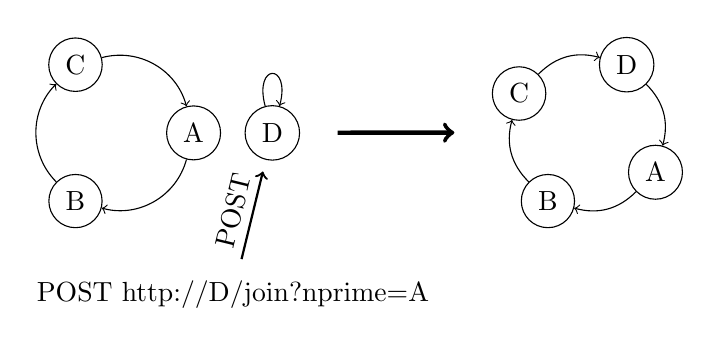
\begin{tikzpicture}[]
                \usetikzlibrary{fit}
                % Draw step 1
                \begin{scope}[every node/.style={circle,draw}]
                    \node (A) at (0:1) {A};
                    \node (B) at (-120:1) {B};
                    \node (C) at (-240:1) {C};
                    \node (D) at (2,0) {D};
                    \draw[->, bend left=45] (A) to (B);
                    \draw[->, bend left=45] (B) to (C);
                    \draw[->, bend left=45] (C) to (A);
                    \draw[->, loop above] (D) to (D);
                \end{scope}
                % Name a node encompassing step 1
                \node[fit=(A) (B) (C) (D)] (step1) {};

                % Create a node for the POST operation text
                \node[anchor=north] (post) at (1.5,-1.75) {POST http://D/join?nprime=A};
                % Draw a slightly thicker arrow from the POST to D
                \draw[->, thick, shorten <=1ex, shorten >=1ex] (post) edge node[above,sloped]{POST} (D);

                % Draw step 2
                \begin{scope}[shift={(6,0)}, every node/.style={circle,draw}]
                    \node (A) at (-30:1) {A};
                    \node (B) at (-120:1) {B};
                    \node (C) at (-210:1) {C};
                    \node (D) at (-300:1) {D};
                    \draw[->, bend left=30] (A) to (B);
                    \draw[->, bend left=30] (B) to (C);
                    \draw[->, bend left=30] (C) to (D);
                    \draw[->, bend left=30] (D) to (A);
                \end{scope}
                % Name a node encompassing step 2
                \node[fit=(A) (B) (C) (D)] (step2) {};

                % Draw a very thick error from step 1 to step 2
                \draw[->, ultra thick, shorten <=1em, shorten >=1em] (step1) to (step2);
            \end{tikzpicture}

            \caption{Using the \textit{/join} call to tell node $D$ to join node $A$'s network.}
            \label{fig:join}

        \end{figure}

    \item[POST /leave]

        Leave the network.
        The node must go back to its starting single-node state,
        and the rest of the network should adjust accordingly.
        How you implement this is up to you.
        The node may notify its neighbors that it is leaving,
        or it can be the network's responsibility to detect the change.

    \item[POST /sim-crash]

        Simulate a crash.
        The node must stop processing requests from other nodes,
        without notifying them first.
        Any request or normal operational messages between nodes should be
        either completely refused or responded to with an error code
        without being acted upon.
        The "crashed" node must respond correctly only to the
        \textit{/sim-recover} and \textit{/node-info} calls.
        The network should detect the crash and respond as if
        the node has left.

        % TODO next year: Disable this /node-info during a crash as well.
        % ONLY /sim-recover should be available.
        % The client can remember which nodes it has crashed.

    \item[POST /sim-recover]

        Simulate a crash recovery.
        The node must "recover" from its simulated crashed state and begin
        responding again to requests from other nodes.
        If the crashed node has been excluded from the network,
        it should request to re-join the network via one of its previous neighbors.

\end{description}

\subsection{Node-Info JSON Format}
\label{node_info_json_format}

The \textit{/node-info} call should return a JSON object similar to the following example:

\begin{lstlisting}[language=Python]
{
    "node_key": "35c25a8",
    "successor": "compute-1-1:8080",
    "others": [
        "compute-2-3:54000"
        ],
    "sim_crash": false
}
\end{lstlisting}

The members are as follows:

\begin{description}

        % TODO next year: be more careful with language for key, id, and hash

    \item[\texttt{node\_key}] (string): the node's hashed key/ID.
        Should be a hexadecimal or integer representation of the hash
        that determines the node's position in the key space.
        If all nodes' keys are put into a list and sorted,
        it should match a list of visiting each node from successor to successor.
        Or, it should for a stable network {(*hint*, *hint*)}.

    \item[\texttt{successor}] (string): the node's successor as a HOST:PORT pair.

    \item[\texttt{others}] (array of strings): the node's other neighbors as a list of HOST:PORT pairs.
        This can include predecessor, finger table members, and any other
        nodes that this node is aware of for any reason.

    \item[\texttt{sim\_crash}] (boolean): true if the node is in a simulated-crash state
        due to a \textit{/sim-crash} call,
        otherwise false.

\end{description}

You can add more info to your \textit{/node-info} response for your own purposes,
but those specified members must be present with the given semantics.

% --------------------------------------------------
\section{Scientific Paper Structure}
\label{scientific_paper_structure}

Scientific papers usually follow a conventional structure, similar to the following.
Try to structure your report similarly.
Use the papers you have read in class as examples.

Scientific Paper Structure:

\begin{description}
    \item[Introduction]
        A brief overview of your solution.

    \item[Background]
        A brief review of concepts necessary to understand your solution (in this case, key-value stores, distributed stores, and distributed hash tables).

    \item[Related Work] A review of other papers related to your work
        (in this case, Chord),
        with notes on how your work differs.

    \item[Description of System (Architecture / Design / Implementation)]
        Actually describe your work.
        Start with a high-level description of the fundamental \textit{architecture} of your solution.
        Then describe other \textit{design} decisions that were made in the process of fleshing out the architecture.
        Finally, describe the low-level \textit{implementation} details
        such as hardware and programming language.

    \item[Evaluation]
        Describe the methods used to evaluate the system.
        Define the metrics used to measure performance,
        and the procedures used to gather metrics.

    \item[Results]
        Give the results of the evaluation, including graphs.

    \item[Discussion]
        Discuss your solution and your experiment results in a more qualitative way. What are the positives and negatives?
        Discuss unexpected results and their implications.

    \item[Future Work]
        Discuss possible ways to improve or expand the system.

    \item[Conclusion]
        Briefly restate the key points of your work and wrap up the paper.

\end{description}

Do not forget to
\begin{itemize}
    \item Make your figures clear and understandable. 
    \item Cite references, insert captions and axes descriptions.
\end{itemize}

\end{document}
